\chapter{Phase behavior of hard aspherical particles}
\label{chap:aspherical}

\section{Introduction}
Problems of packing and space tiling have fascinated scientists for a very long time.
Kepler's 1611 essay {\it ``Strena Seu de Die Nive Sexangula''} (``A New Year's Gift of Hexagonal Snow'')~\cite{Kepler} is probably one of the earliest publications on the subject.
Herein he conjectured that cubic close packing and hexagonal close packing are the most efficient ways to fill a space using equally sized spheres.
It wasn't until 1998 that Kepler's conjecture was finally announced to be proven (with a 99\% degree of confidence) by Thomas Hales~\cite{Hales}.

Most of the work on particle crystallization and self-assembly in the last decade has focused on monodisperse~\cite{frenkel1} or polydisperse~\cite{frenkel2,zaccarelli} systems of spherical or regularly-shaped particles (see also~\cite{glotzer,chandler,geissler,cacciuto,torquato,frenkel,glotzer2,glotzer3,glotzer4,esco,weitz} and references therein).
Nevertheless, there are several important cases in which the shape of the single components cannot be tailored at will; however, an efficient packing, or an understanding of the physical properties of these densely compressed systems, is highly desirable.
Two examples of outstanding problems in this category are the storage of grains~\cite{deGennes} and protein crystallization~\cite{rosenberger}.
Both examples can be ideally thought of as two different aspects of the problem of understanding the role of shape in particle packing.
In the first case the goal is to efficiently pack a system of randomly-shaped polydisperse grains; 
in the second, the aim is to crystallize non-spherical, yet equally shaped monodisperse components. 
In this chapter, both of these cases will be addressed. 

An understanding of the relationship between the ability of particles to form macroscopically-ordered crystal structures and their shape is sought.
Specifically, we analyze how random perturbations from the ideal spherical shape affect the crystallizability of a densely packed system of indistinguishable hard particles.
Although a few papers have  dealt with the thermodynamic behavior of soft/deformable particles as a model for polymer brushes or polymer-coated colloids (\cite{pamies,capone,richter,bozorgui} and references therein), this is the first study where shape distortions, frozen onto the particles, are explicitly and systematically accounted for.

Crystallization in these systems occurs because of the free volume gain associated with the crystal structure, as discussed in Section~\ref{sec:CNT}.
However, even in simple systems, precise calculations of the free energies involved in these transitions are very difficult. 
In complicated systems such as those discussed in this chapter, it is implausible to perform these calculations rigorously, and since the transition depends on small differences between large free energy values, computer simulations are the tool of choice to study and analyze this important process in detail.

\comment{The problem of crystal formation is poorly understood.
From a thermodynamic standpoint, classical nucleation theory informs us that a crystal can only be formed via a barrier crossing event.
The free energy gain to form a nucleus of a stable crystalline structure in a supersaturated solution must balance out the free energy cost associated with the formation of an interface between the solid and the fluid parent phase.
The Gibbs free energy cost, $\Delta G$, associated with this event has a strong dependence on the interfacial free energy, $\gamma$: ${\Delta}G \propto \frac{\gamma^3}{(\rho\Delta\mu)^2}$,  where $\rho$ and $\Delta\mu$ are the density and the chemical potential difference between solid and fluid phase, respectively.
As $\gamma$ is very hard to extract from experiments, computer simulations are the tool of choice to study and analyze this important process in detail.}

\section{A model of hard aspherical particles}\label{sec:asphermethod}
In this chapter, each particle is built by randomly setting the center of $N_b$ ($4 \leq N_b \leq 12$) spheres of diameter $\sigma$ inside a spherical shell of diameter  $\sigma_0<\sigma$.
The overall volume generated from the resulting overlapping aggregate defines our new particle.

Deviations from the ideal spherical shape can be conveniently controlled by varying $\sigma_0$ and $N_b$. 
For  $\sigma_0=0$ one recovers the spherical limit, and as  $\sigma_0$ increases, particles develop larger and larger shape distortions.
In a similar fashion, large values of $N_b$ result in a bumpy but overall isotropic particle, whereas small values of $N_b$ tend to generate very anisotropic shapes.

Once a particle is built, the center of mass of this cluster of balls is determined, and the entire cluster is scaled so that its total volume equals that of a spherical particle of diameter $\sigma$, i.e. $\frac{\pi}{6}\sigma^3$.
Any two particles $i$ and $j$ interact via a hard repulsive potential defined as
\begin{equation}
U_{ij}=
\begin{cases}
0 & {\textrm{if }} |r_s-r_t|>\sigma_R \,\,\,\,\,\,\forall s\in i \,\,,\,\, \forall t\in j \cr
\infty &\text{otherwise}\cr
\end{cases} \,,
\end{equation}
where $s$ and $t$ run over all spheres of rescaled diameter $\sigma_R$ constituting particle $i$ and particle $j$ respectively.
Experimental realizations of colloidal particles similar to ours could be generated using the approach described in~\cite{weitz} to create uniform nonspherical particles with tunable shapes.  

Figure~\ref{shapes} shows a few snapshots of particle shapes obtained for different values of $N_b$ and  $\sigma_0$.
In Section~\ref{sec:polydisperse}, a specific $N_b$ and $\sigma_0$ will be chosen and a system will be composed of different random particles generated using the method above with those two parameters as inputs; in Sections~\ref{sec:disorderpress} and~\ref{sec:disorderyesno}, a system will be made up of identical particles from one specific outcome of the particle generation procedure.
\begin{figure}
	\begin{center}\includegraphics[width=0.8\textwidth]{disorder/parts2.png}\end{center}
	\caption[Model particles for different values of $\sigma_0$ and $N_b$]{Model particles for different values of $\sigma_0$ and $N_b$ built according to the scheme described in the text.}\label{shapes}
\end{figure}

Two order parameters characterizing the degree of asphericity of a particle are useful for relating the shape of particles in a system. 
The first is its asphericity, $A$ (as opposed to the commonly used sphericity, $S$~\cite{sphericity}), defined in terms of the surface to volume ratio of a particle $\alpha_p=\frac{A_p}{V_p}$ with respect to that of a sphere of diameter $\sigma$, $\alpha_s=\frac{6}{\sigma}$, as
\begin{equation}
	A = 1 - S = 1-\frac{\alpha_s}{\alpha_p} \,.
\end{equation}
Given our model setup, $V_p=V_s$, $A$ simplifies to 
\begin{equation}
	A=1-\frac{\pi\sigma^2}{A_p} \,.
\end{equation}

The surface area of a particle, $A_p$, is calculated via a simple Monte Carlo algorithm: a random point on the surface of a random one of the $N_b$ spheres is chosen, and it is determined whether it is inside any of the other spheres or not -- only points which do not lie on the inside of any other sphere are on the surface of the overall particle.
This is repeated until the proportion of points on the surface of the particle as a fraction of all points chosen converges; using this fraction and the total surface area of all of the spheres combined, $N_b \times \pi \sigma_R^2$, the surface area of the particle can be calculated.
 
The second parameter, $q$, measures the orientational symmetry  of the particle.
It is used to describe the  asphericity of random walks~\cite{rudnick}, and it is obtained by combining invariants of the particle inertia tensor $I_{ij}$  as
\begin{equation}
	q=\frac{\left(R_1^2-R_2^2\right)^2 + \left(R_1^2-R_3^2\right)^2 + \left(R_2^2-R_3^2\right)^2}{2\left(R_1^2 + R_2^2 + R_3^2\right)} \,,
\end{equation}
where $R_1$, $R_2$, and $R_3$ are the three principal eigenvalues of the inertia tensor of the particle, that is, the three principle radii of gyration of the particle.

Both parameters are defined so that they are equal to $0$ for a perfectly spherical particle, and approach $1$ for  extremely aspherical ones. 
Note that $A$ depends intimately on the value of $\sigma_0$ used to construct the particle, whereas $q$ depends only on the angular distribution of spheres about the center of mass -- that is, it is completely independent of $\sigma_0$.

It is worth briefly describing the limits of $q$, in particular, as its definition is less intuitive than that of $A$.
As defined, the $q \rightarrow 0$ limit is a sphere; $q \simeq \frac{1}{2}$ for a thin, circular plate; and $q \rightarrow 1$ for a long, thin rod.

\section{Shape-polydisperse systems}
\label{sec:polydisperse}
\comment{\subsection{Introduction}

Understanding how objects pack or can be designed to tile the three dimensional space is a fundamental optimization problem that has important practical applications that
range from the macroscopic, such as the efficient storage of grains,  to the microscopic: the fabrication of band-gap photonic materials.
Mathematicians have been intrigued by such problems for centuries; namely since Kepler's 1611 essay {\it On the Six-cornered Snowflakes}, but it wasn't 
until recently, with the advent of nanotechnology and the explosion of molecular biology, that problems of packing and self-assembly of nanoscopic components 
gained   tremendous traction in the broader scientific community.   
Recent advances in synthesis of nanoparticles~\cite{DeVries,Schnablegger,Hong,Weller,Hobbie,weitz,pine,mitragotri} allowed for unprecedented control over the 
 shape and surface chemistry of colloidal particles, thus providing an unlimited number of building blocks whose 
 spontaneous aggregation could lead to the formation of an unprecedented variety of structures with potentially novel functional, mechanical, and optical properties.
 Unlike most of the work on particle crystallization and self-assembly that in the last decade has focused on 
 monodisperse~\cite{frenkel1} or polydisperse~\cite{frenkel2,zaccarelli} systems of spherical or regularly-shaped particles  (see also~\cite{glotzer,chandler,geissler,cacciuto,torquato,frenkel,glotzer2,glotzer3,glotzer4,esco,weitz} and references therein), surprisingly little or nothing has been done
 theoretically to understand the packing of irregularly shaped particles. 
Indeed, there are several important cases in which the shape of the single components cannot be tailored at will,
 yet, an efficient packing, or an understanding of the physical properties of these densely compressed systems, is highly desirable.
Two examples of outstanding problems in this category are the storage of grains~\cite{deGennes} and protein crystallization~\cite{rosenberger}.
Both examples can be ideally thought of as two different aspects of the problem of understanding the role of shape in particle packing: systems of either polydisperse or indentically-shaped (monodisperse) components. 
  
Here we seek to gain insight into the crystallization of nonspherical particles. 
 We want to understand how  particle geometric features can be related to their ability to orderly pack into three dimensional periodic structures,
 and especially  to identify under what conditions they cease to do so. 
 We have recently reported~\cite{disorder1}  that it is possible to empirically relate particle geometry to crystallizability (intended as the tendency of a component to crystallize) 
by using two simple geometric parameters. The first is the particle asphericity  $A$, defined in terms of the 
surface to volume ratio of a particle $\alpha_p=A_p/V_p$ with respect to that of a sphere of diameter $\sigma$, $\alpha_s=6/\sigma$, as
$A =1-\alpha_s/\alpha_p.$  The second parameter, $q$, is related to the  orientational symmetry  of the particle.
It is used to describe the  asphericity of random walks~\cite{rudnick}, and it is obtained by combining invariants of the particle inertia tensor $I_{ij}$  as
$q=\sum_{i< j} (\lambda_i^2-\lambda_j^2)^2/\sum_i \lambda_i^2$, where $\lambda_i$, with $i=1, 2, 3$, is an eigenvalue of $I_{ij}$.
 
In this paper we try to rationalize those empirical results by computing how random perturbations from the ideal spherical 
shape affect the fluid-solid coexistence pressure of  monodisperse and shape-polydisperse systems of hard aspherical particles.

In order to generate a  statistical ensemble of aspherical particles, we developed a simple model~\cite{disorder1} that guarantees a certain degree of control over
the particle shape. Each particle is built by setting the center of $N_b$ ($4 \leq N_b \leq 12$) spheres of diameter $\sigma$ at random 
positions on the surface a spherical shell of diameter $\sigma_0<\sigma$.
The overall volume generated from the resulting overlapping aggregate defines our new particle.
Polydisperse systems of such aspherical particles were generated by choosing specific values of $N_b$ and $\sigma_0$ and allowing each particle in the system to arise from a different random collection of sphere positions.
Deviations from the ideal spherical shape can be conveniently controlled by varying $\sigma_0$ and $N_b$.
For  $\sigma_0=0$ one recovers the spherical limit, and as  $\sigma_0$ increases, particles develop larger and larger shape distortions.
In a similar fashion, large values of $N_b$ result in a bumpy but overall isotropic particle, whereas small values of $N_b$ tend to generate very anisotropic shapes.
Once a particle is built, the entire cluster is scaled so that its total volume equals that of a spherical particle of diameter $\sigma$, i.e. $\frac{\pi}{6}\sigma^3$.
Any two particles $i$ and $j$ interact via a hard repulsive potential defined as
\begin{equation}
U_{ij}=
	\begin{cases}
		0 & {\textrm{if }} |r_s-r_t|>\sigma_R \,\,\,\,\,\,\forall s\in i \,\,,\,\, \forall t\in j \cr
		\infty &\text{otherwise}\cr
	\end{cases}
\end{equation}
where $s$ and $t$ run over all spheres of rescaled diameter $\sigma_R$ constituting particle $i$ and particle $j$ respectively.
Experimental realizations of colloidal particles similar to ours could be generated using the approach described in reference~\cite{weitz,pine,mitragotri} 
to create nonspherical particles with tunable shapes. }

The results of simulations of polydisperse systems will be presented first.
Such systems could represent, for example, a system of colloidal particle which is ``sloppily'' synthesized with some tolerance for deviation from a perfect sphere.
Polydisperse systems have one major advantage, for a study such as that described below, over monodisperse systems: statistics.

In order to build up the statistical basis necessary to relate order parameters such as those described in Section~\ref{sec:asphermethod}, a large number of systems must be simulated for each data point; this severely limits the computational cost that may be expended per system.
Polydisperse systems represent a huge decrease in the number of independent variables; because each system is made up of a large number of different particle shapes, one may be confident that the result obtained is not a result of some peculiarity of a specific shape studied.
In Sections~\ref{sec:disorderpress} and~\ref{sec:disorderyesno}, monodisperse systems are studied, both as a comparison with the results attained in this section as well as using less computationally-intensive methods in order to study a larger number of particle shapes.

In order to determine the fluid-solid coexistence pressures for systems of aspherical particle, the method of direct fluid-solid coexistence simulation described in~\cite{noya} was used.
1024 particles were placed in an fcc crystal lattice (at volume density $\rho_s \simeq 0.545$, the hard sphere crystal coexistence density~\cite{HScoex}) centered in a box of dimensions $L_x \times L_y \times L_z$.
An fcc crystal was chosen based upon preliminary work, which indicated that when monodisperse aspherical systems form crystals, they tend to be (apart from a very few particular exceptions) fcc; no evidence has been found supporting the use of any other crystal geometry.

The dimensions of the box were chosen such that $L_x$ and $L_y$ were just large enough to accomodate the fcc crystal, and $L_z$ was roughly four times larger.
The crystal lattice was chosen such that the extension of the crystal in the $z$-direction was roughly twice that in the $x$- and $y$-directions, in order to increase the separation between the two fluid-solid interfaces in the system; by decreasing the surface-to-volume ratio of the crystal, one hopes to come as close to a ``bulk-like'' system as possible.

This crystal lattice was placed into equilibrium with a fluid of 1024 particles at hard sphere fluid coexistence volume density $\rho_l \simeq 0.495$.
The fluid and crystal were both briefly allowed to relax in order to relieve any overlap introduced by the ``bumpiness" of the particles and to allow the fluid to come fully into contact with the solid interface; because the particles are hard, there must be zero overlap in between particles.

Monte Carlo simulations were then run with constant number of particle $N$, pressure $p$, and temperature $T$ ($NPT$ ensemble), where the three box dimensions $L_x$, $L_y$, and $L_z$ were allowed to fluctuate independently under the isotropic pressure $p$.

The number of crystalline particles, $N_X$, in the system was monitored as a function of Monte Carlo step; this quantity was determined using the standard spherical-harmonics based bond order parameter $q_6$ described in Section~\ref{sec:orderparamdesc}.
Simulations were performed starting from a system initialized as desribed above, and $N_X$ was monitored over the course of the simulation to determine whether it decreased (crystal melting) or increased (crystal growth).

Below the coexistence pressure, the crystal will melt, and above it, the crystal will grow; thus, the pressure at which the system transitions (as a function of pressure) from decreasing $N_X$ to increasing $N_X$ represents the coexistence pressure $p^*$.
This method is known to have a few caveats: slow equilibration, non-negligible finite size effects,  dependence of the surface free energy on the specific face the crystal exposes to the fluid~\cite{noya}.
Nevertheless, for this specific system, we find this direct  method to be  more reliable than the two-step thermodynamic integration scheme described in~\cite{dijkstra}. 

\comment{\begin{figure}
	\begin{center}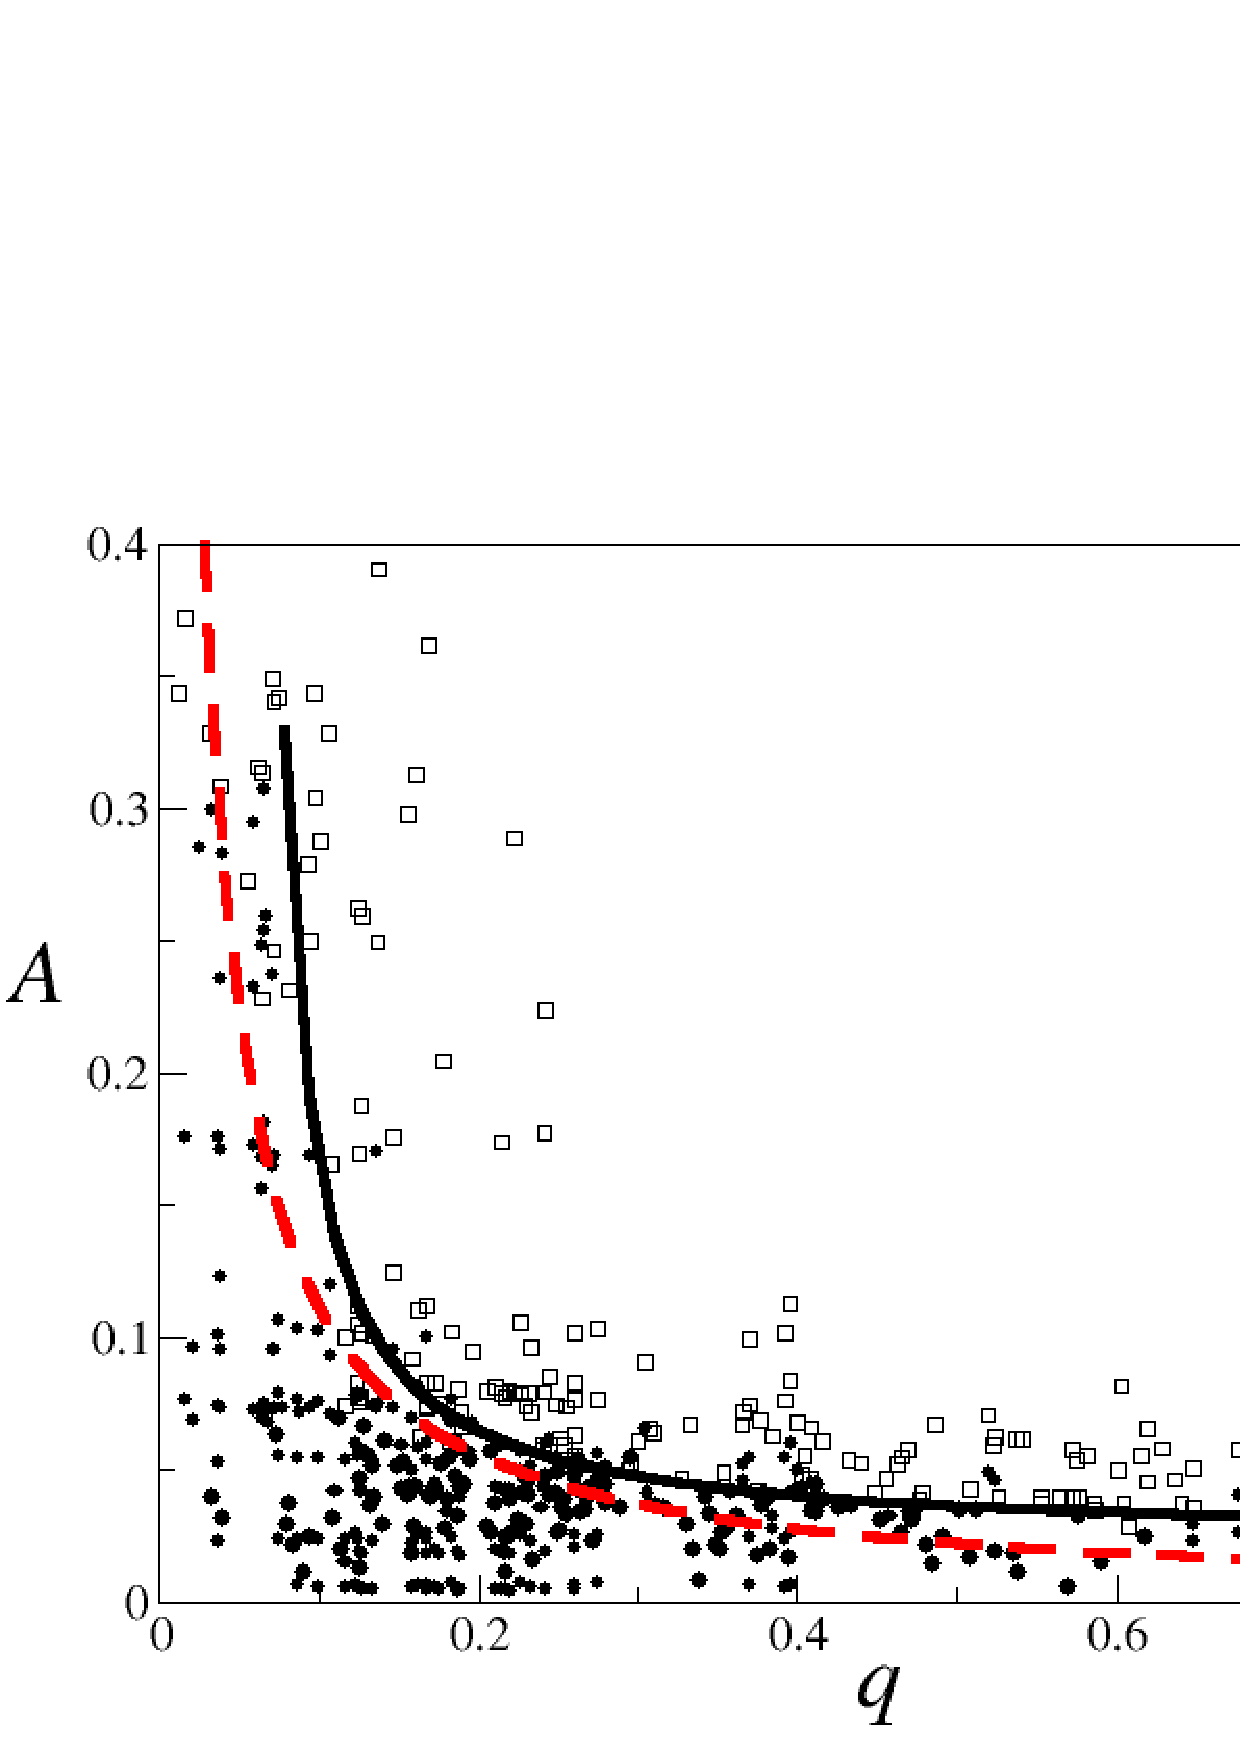
\includegraphics[width=0.8\textwidth]{polydisperse/mono1.png}\end{center}
	\caption[Crystallizability of monodispers aspherical particles vs. $A$ and $q$]{Crystallizability of monodisperse aspherical particles characterized in terms of two shape parameters $A$ and $q$. Filled circles indicate particles that easily crystallized, while open squares indicate particles that did not.  The dashed line represents a prediction of the crystallizability limit from the current work; see below.  Figure adapted from~\cite{disorder1}.}\label{mono1}
\end{figure}
Our empirical results on the crystallizability of   systems of monodisperse aspherical particles ~\cite{disorder1}, obtained by slowly compressing an ensemble of 487 different shape realizations
 are summarized in  Fig.~\ref{mono1} and indicate the existence of a clear boundary between particles that crystallize and particles that do not.
  A roughly inverse relationship is clearly evident; particles with large $A$ must have very small $q$ in order to have
a hope of crystallization, and vice-versa. This result provides a very useful way of predicting whether a particular particle shape can pack into a
crystalline structure by simply measuring the experimentally accessible $A$ and $q$. 
As this  model is intended to describe randomly shaped particles, the diagram does not include the results for particles designed with very specific shapes such as rods,
plates or regular polyhedral geometries that are known to crystallize. 
These particular cases would generate sharp peaks around specific values of $q$, and are purposefully excluded from this study.
 The solid line is  a guide to the eye and has the functional form $A(q) = 0.023 + 1/(170q-10)$.} 

Incorporating shape-polydispersity in these systems is not a trivial matter and requires some discussion.  
Unlike the common notion of polydispersity of spherical particles  for which any particle size can be indifferently used as a reference (and thus only the width, not the center, of the distribution matters), each particle shape could be used as a reference shape for this study. 
The problem is that the phase behavior could be very much dependent on the specific choice of $A$ and $q$.
We therefore adopted a pragmatic approach to describing shape-polydispersity  that has a natural experimental counterpart~\cite{weitz}. 

\begin{figure}
	\begin{center}
		\subfloat[]{\includegraphics[width=0.6\textwidth]{polydisperse/Ahist.png}\label{Ahist}}

		\subfloat[]{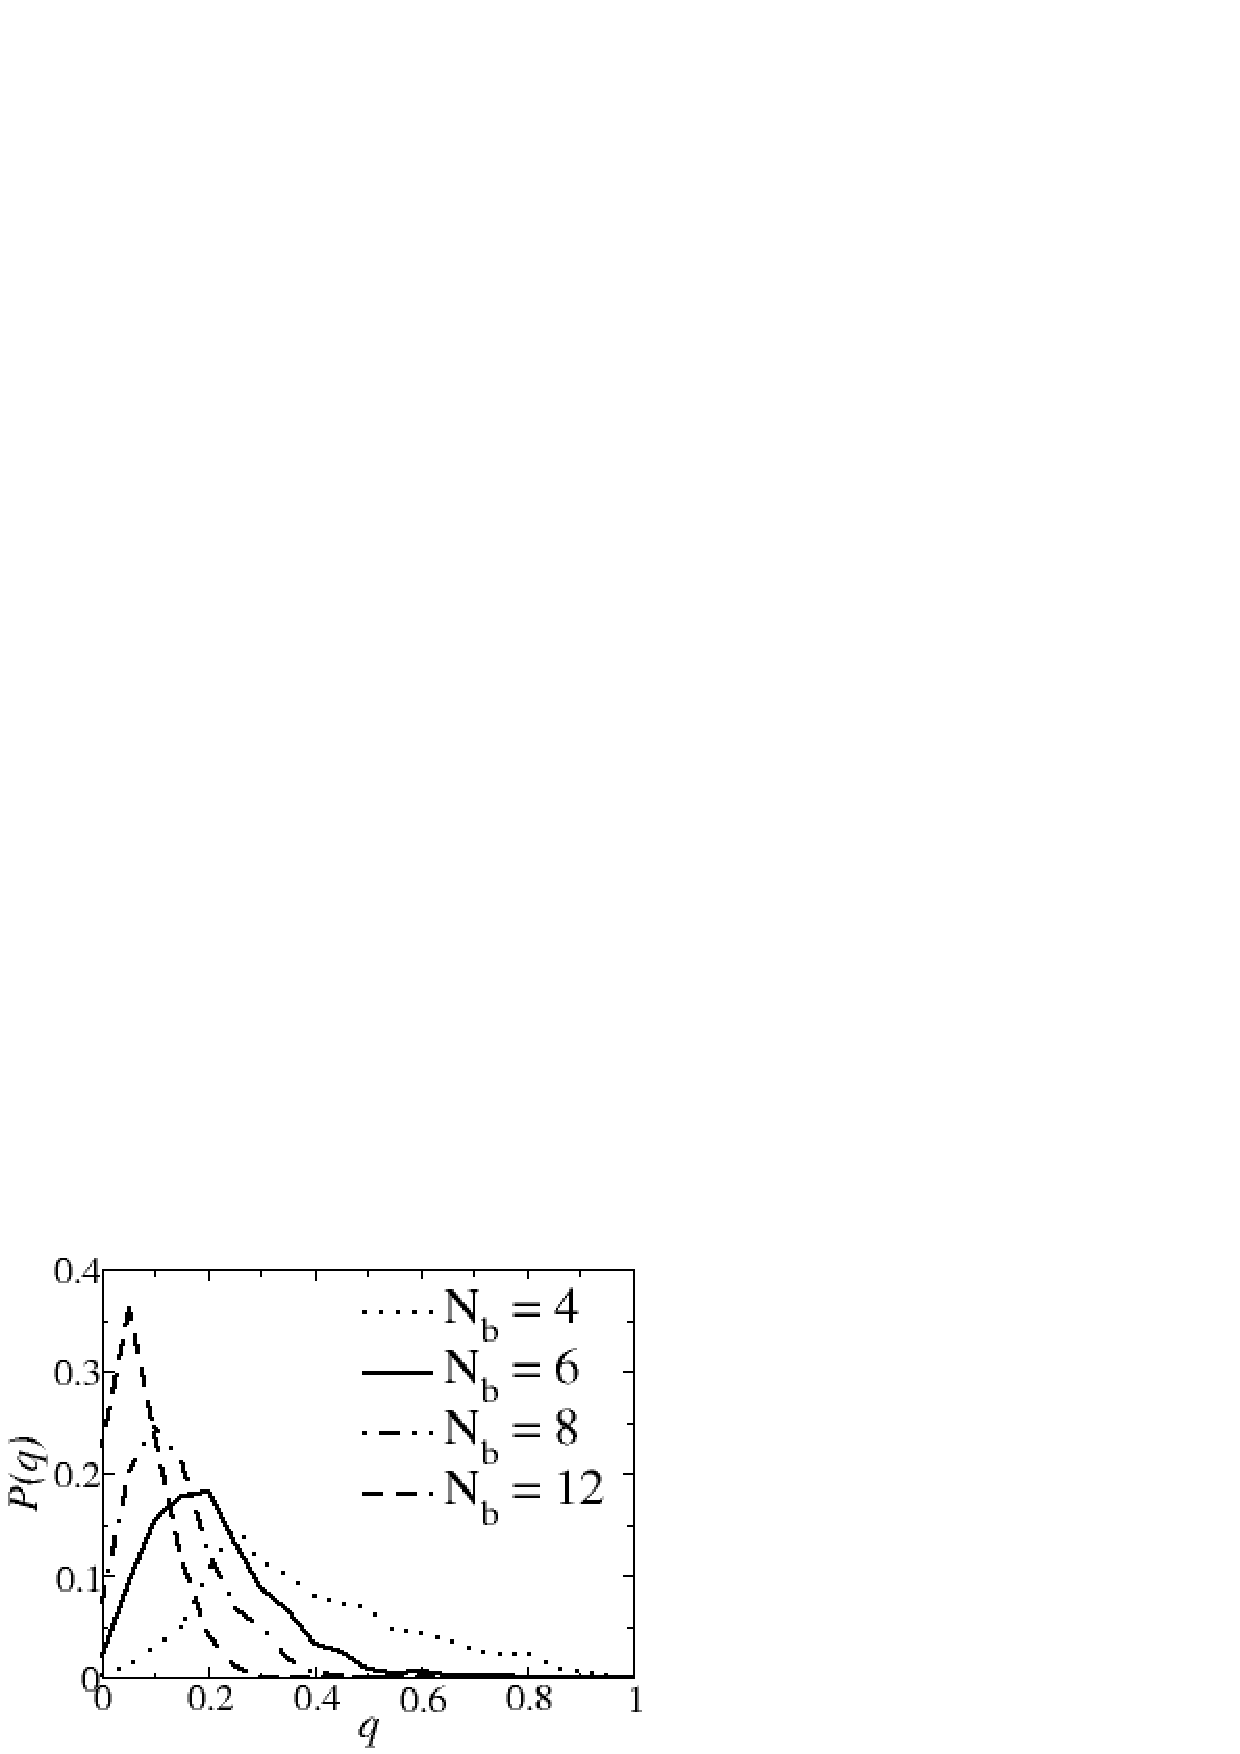
\includegraphics[width=0.6\textwidth]{polydisperse/qhist.png}\label{qhist}}
	\end{center}
	\caption[$A$ and $q$ distributions for different values of $\sigma_0$ and $N_b$]{\subref{Ahist} Probability distributions of $A$ for polydisperse systems with $N_b = 8$ and various values of $\sigma_0 \in [0.05,0.30]$.  the $A$ distribution is approximately independent of $N_b$.  \subref{qhist} Distribution of $q$ values for polydisperse systems with $N_b$ = $4$, $6$, $8$, and $12$.  Recall that $q$ is independent of $\sigma_0$.  The distribution is significantly larger and broader for $N_b = 4$ than for the larger values of $N_b$.}\label{histograms}
\end{figure}

Namely, we  consider the distributions of $q$s and $A$s arising when constructing our particle using a given number of spheres $N_b$ and a given value of $\sigma_0$.
Particles  with large values of $N_b$ generate narrow distributions shifted towards small values of $q$, while small values of $N_b$ ($N_b\geq 4$) result in wide distributions peaked over large values of $q$.
When $\sigma_0\rightarrow 0$ one recovers the  hard sphere limit for any value of $N_b$, and as $\sigma_0$ increases,  larger and larger values of $A$ will be sampled (without affecting the $q$ distributions) until approaching the crystallizability boundary.
Sample distributions of $A$ and $q$ for varying values of $\sigma_0$ and $N_b$ (respectively) are shown in Figure~\ref{histograms}

We systematically analyzed particles constructed with $N_b =4$, $5$, $6$, $8$, and $12$, and values of  $\sigma_0 \in[0.05,0.30]$.

\begin{figure}
	\begin{center}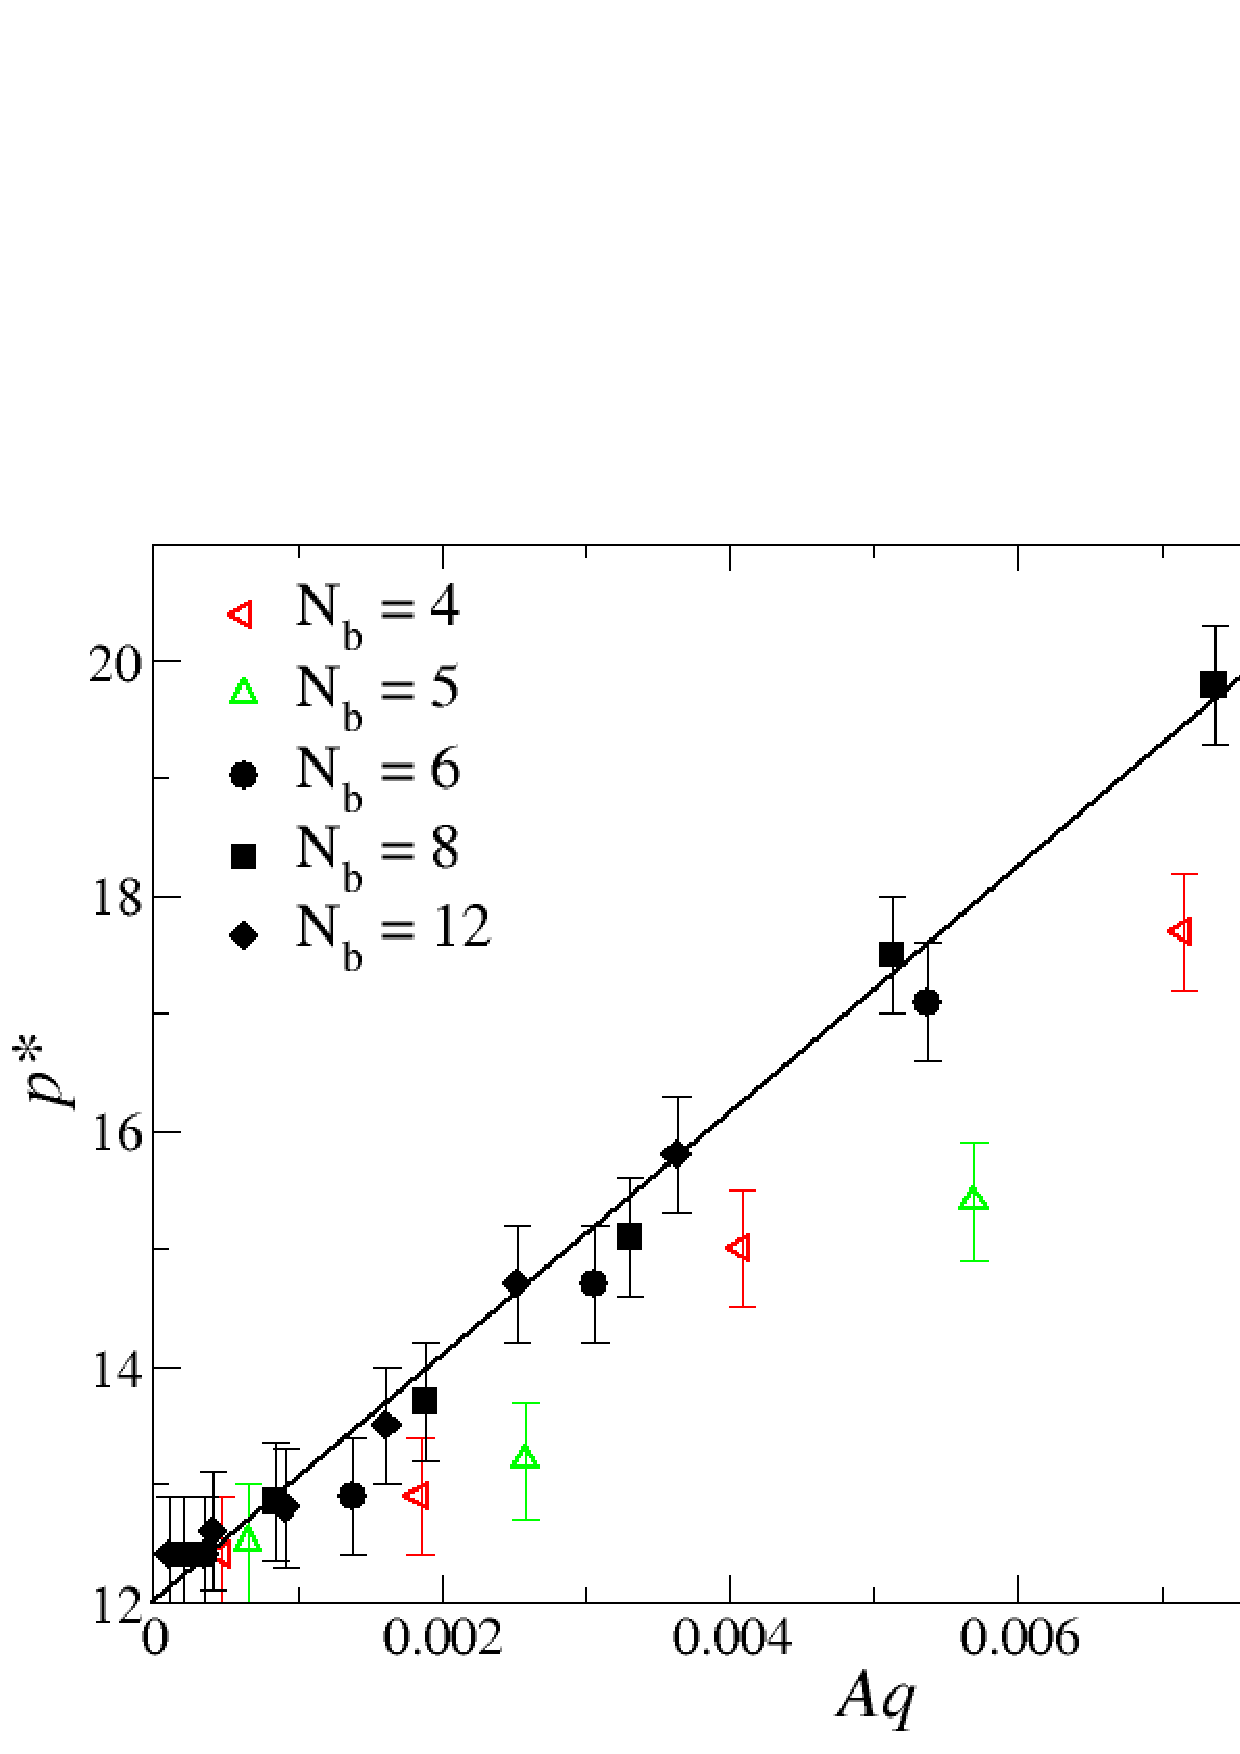
\includegraphics[width=0.8\textwidth]{polydisperse/poly.png}\end{center}
	\caption[Coexistence pressures for shape-polydisperse systems vs. $Aq$]{Coexistence pressure vs. $Aq$ for shape-polydisperse systems of hard aspherical particles. The solid line is a fit to the data for $N_b\geq 6$.}\label{poly}
\end{figure}
All data points have been computed using two different random sets of particle geometries from the given distribution.
The difference between the results from the two independent sets is smaller than the error bar associated with the numerical scheme.
Figure~\ref{poly} shows our results: the coexistence pressure $p^*$ (as defined above) versus the product $Aq$ for $4 \leq N_b \leq 12$ and $\sigma_0 \in [0.05,0.30]$.

Unsurprisingly, the coexistence pressure increases with increasing $A$ and $q$, but remarkably, for $N_b \geq 6$, the relationship between $p^*$ and $Aq$ is simple linear one.
We find that the coexistence pressures for these $N_b$ values  be fitted to  $p^* (A,q)= 991Aq + 12$.
Note that the y-intercept is near the hard sphere coexistence pressure of $p^*_{\rm HS}\simeq  11.7$~\cite{HScoex}, as it should be.
This should be expected because the $Aq \rightarrow 0$ limit is a system of hard spheres.

These results thus suggests that $p^*(A,q)$ can be expressed in terms of a Taylor expansion in the quantity $Aq$: 
\begin{equation}
	\frac{p^*(A,q)-p^*_{\rm HS}}{p^*_{\rm HS}} = \alpha Aq + ...
\end{equation}
Note, however, that significant but systematic deviations from the linear fit are visible for systems of particles obtained with  $N_b = 4$ and $N_b = 5$. 
These values of $N_b$ correspond to particles with  relatively large values of $q$ and rather broad distributions (see Figure~\ref{qhist}), suggesting that other, higher-order terms in the expansion may be necessary. 
Furthermore, for such wide distributions fractionation  between isotropic and anisotropic particles may become an important factor -- this is an effect to which the direct simulation method used here is completely blind, because the system is initialized with a preformed crystalline volume with a random selection of particles.
Fractionation would require complete melting of the initial crystal and subsequent formation of a fractionated crystal, which was not allowed in this study.

\section{Monodisperse systems: coexistence pressures}\label{sec:disorderpress}
\begin{figure}
	\begin{center}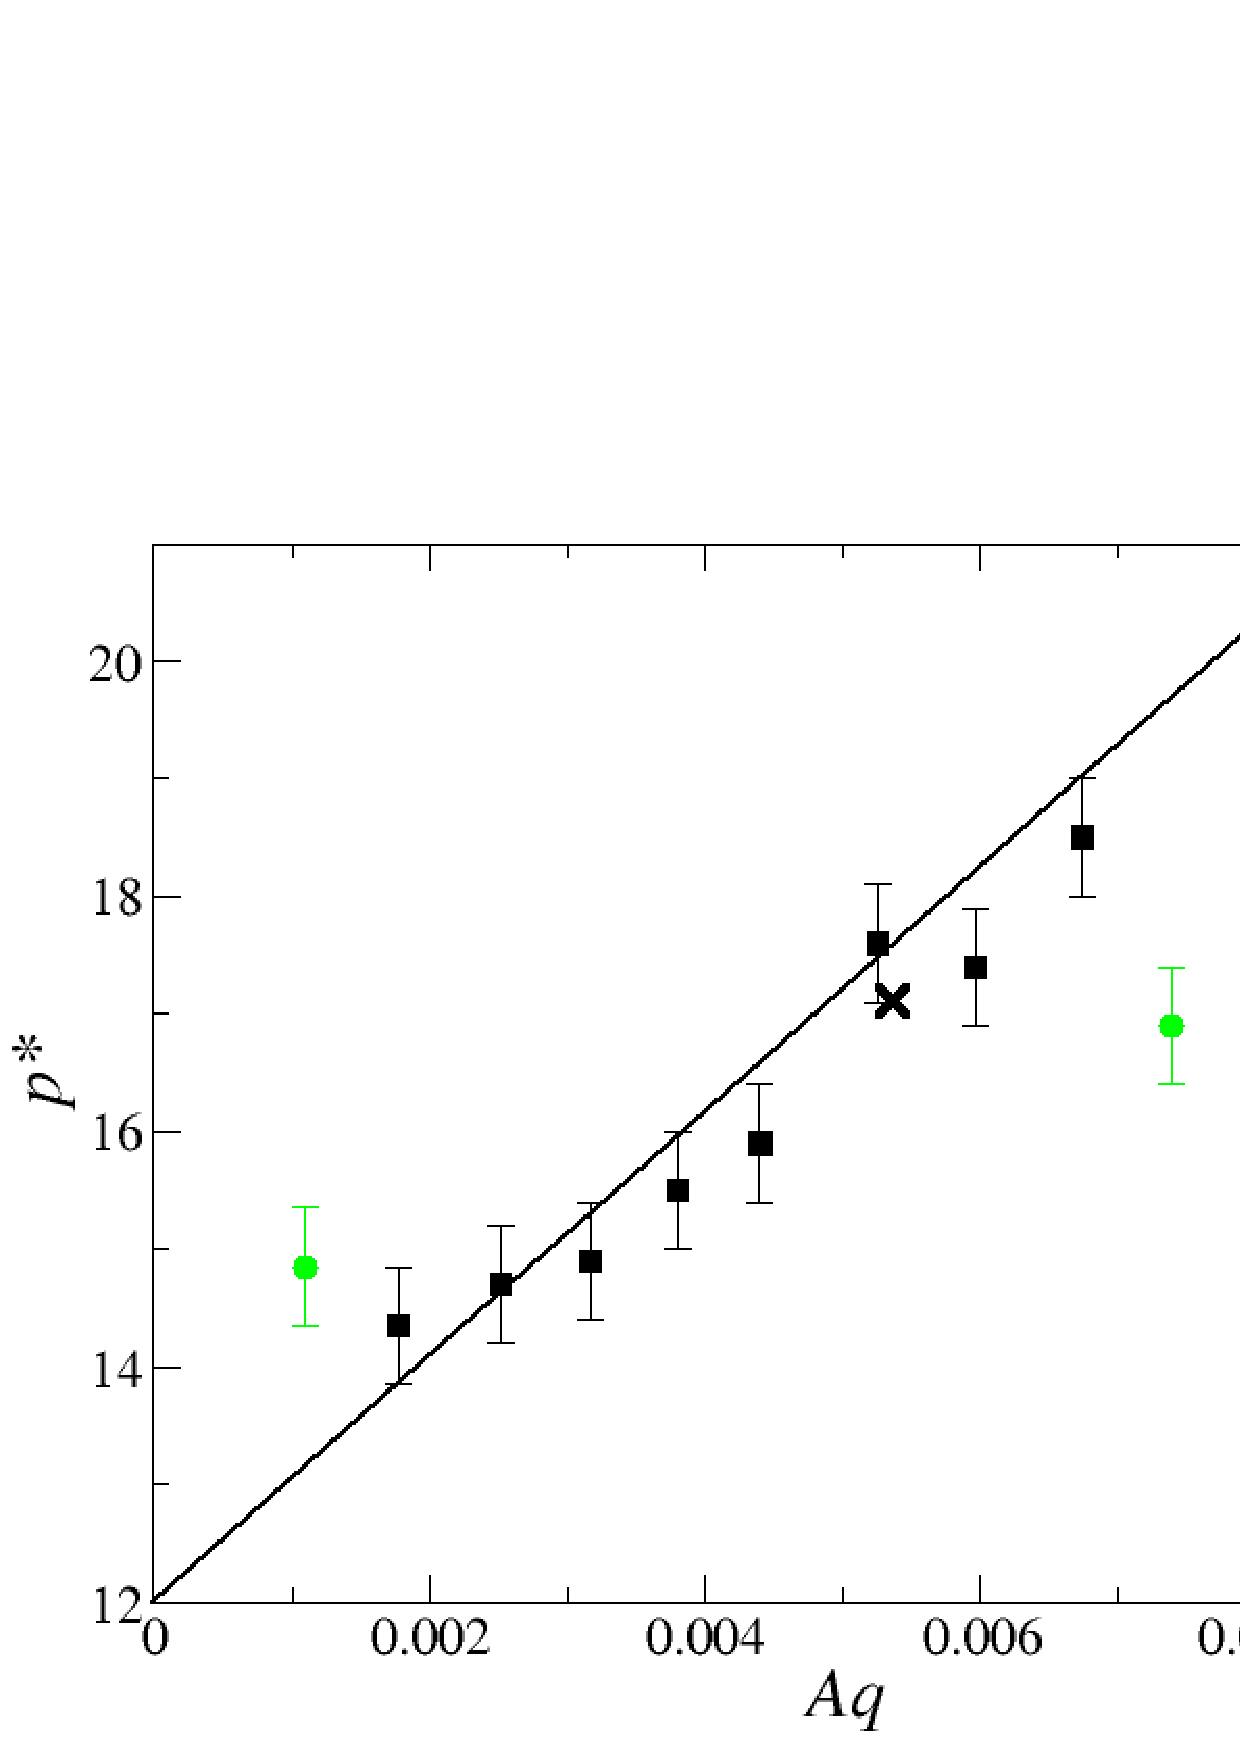
\includegraphics[width=0.8\textwidth]{polydisperse/mono2.png}\end{center}
	\caption[Coexistence pressure vs. $Aq$ for monodisperse systems of aspherical particles]{Coexistence pressure vs. $Aq$ for monodisperse systems of hard aspherical particles with $N_b = 6$, $\sigma_0 = 0.2$.  The line is a fit obtained from the data presented in Figure~\ref{poly} for polydisperse systems with $N_b = 6$, $8$, and $12$.  The cross indicates the position of the polydisperse system with $N_b = 6$, $\sigma_0 = 0.2$.
Points at the extremes of the $q$ distribution are shaded with a lighter color.}\label{mono2}
\end{figure}

The existence of a master curve for the coexistence pressure of significantly different particle distributions (provided $N_b\geq6$), both in terms of their average value  and their width, is quite remarkable, and provides a very compact and elegant way of expressing the equilibrium properties of such systems.  
As a test of the robustness of this relationship, ten monodisperse systems were generated by a single set of parameters: $N_b = 6$, $\sigma_0 = 0.2$.
Each of these systems is characterized, by definition, by an infinitely sharp $P(q)$, and individual configurations were selected to cover a fairly wide range of $Aq$ values, while keeping $A$ roughly constant (because the distribution of $A$ values for a given set $(N_b,\sigma_0)$ is narrow, see Figure~\ref{Ahist}). 
A plot of these data, shown in Figure~\ref{mono2}, indicates that the relationship adapted unaltered from the polydisperse case is a reasonably good predictor of coexistence pressure for the monodisperse case as well.
This is a clear indication that, up to some maximum, the master curve is overall independent of distribution width.

Notice that no coexistence pressures above $p^*(A,q) \simeq 21$ are reported. 
This is not a coincidence; in general, if a system was going to crystallize at all (that is, if the crystalline region of the simulation box was going to grow), the coexistence pressure $p^*$ was below this value.
This is interesting because this value is close to the fluid pressure of a system of hard spheres
at the glass transition density~\cite{speedy}, $p_G = 22.6$, and  it is reasonable to assume that $p_G$ sets an upper bound to the 
largest accessible fluid coexistence pressure for aspherical particles obtained with direct fluid/solid sampling.

In fact, this method  
is clearly susceptible to anomalies in system kinetics, thus making coexistence measurements at pressures larger than the ones herein reported 
quite cumbersome and somewhat unreliable. Nevertheless, if we assume that no aspherical hard particle will easily crystallize above $p_G$, we can 
formulate a prediction for whether a system of aspherical particles should be expected to easily crystallize: given $p^* \simeq 991 Aq + 12$, and based upon this simple line of reasoning, one should expect, as a first-order approximation, a limit of
\begin{equation}Aq \lesssim 0.011 \,.\label{xtallimit}\end{equation}
When the product $Aq$ is below this limit, the system would be expected to easily crystallize at some pressure; above the limit, the system is never expected to crystallize.

\section{Monodisperse systems: predicting crystallization}\label{sec:disorderyesno}

In order to test the prediction above, a large number of monodisperse systems was tested for the simple binary question: ``Does this system crystallize easily?''
In order to answer this question, traditional Monte Carlo simulations were performed in the $NPT$ ensemble.
Instead of intializing the system to be half crystalline and half fluid, a cubic box was used and the simulations was initialized in a fluid state.
Each simulation contained $N = 128$ particles and contained a monodisperse system of aspherical particles constructed with some value of $(N_b, \sigma_0)$; for the purposes of this study, we used $N_b \in \left\{4,6,8,12\right\}$ and $\sigma_0 \in \left(0,1\right)$.

The initial pressure was set to $p = 10$ and the pressure was incremented by $\Delta p = 0.5$ or smaller.
Each simulation was run for a minimum of $4 \cdot 10^6$ Monte Carlo sweeps after thermalization.
The simulation was ended when the system either crystallized or reached a volume fraction $\phi \simeq 0.6$, above the glass transition point of hard sphere, $\phi_G = 0.58$.
Crystallization was detected by a combination of (a) the $q_6$ order parameter, (b) a careful monitoring of the system volume fraction over time for sudden jumps (indicating a phase transition), and (c) visual inspection.
We investigated a total of $487$ different particle geometries. 

Figure~\ref{mono1} summarizes the result of this study. 
\begin{figure}
	\begin{center}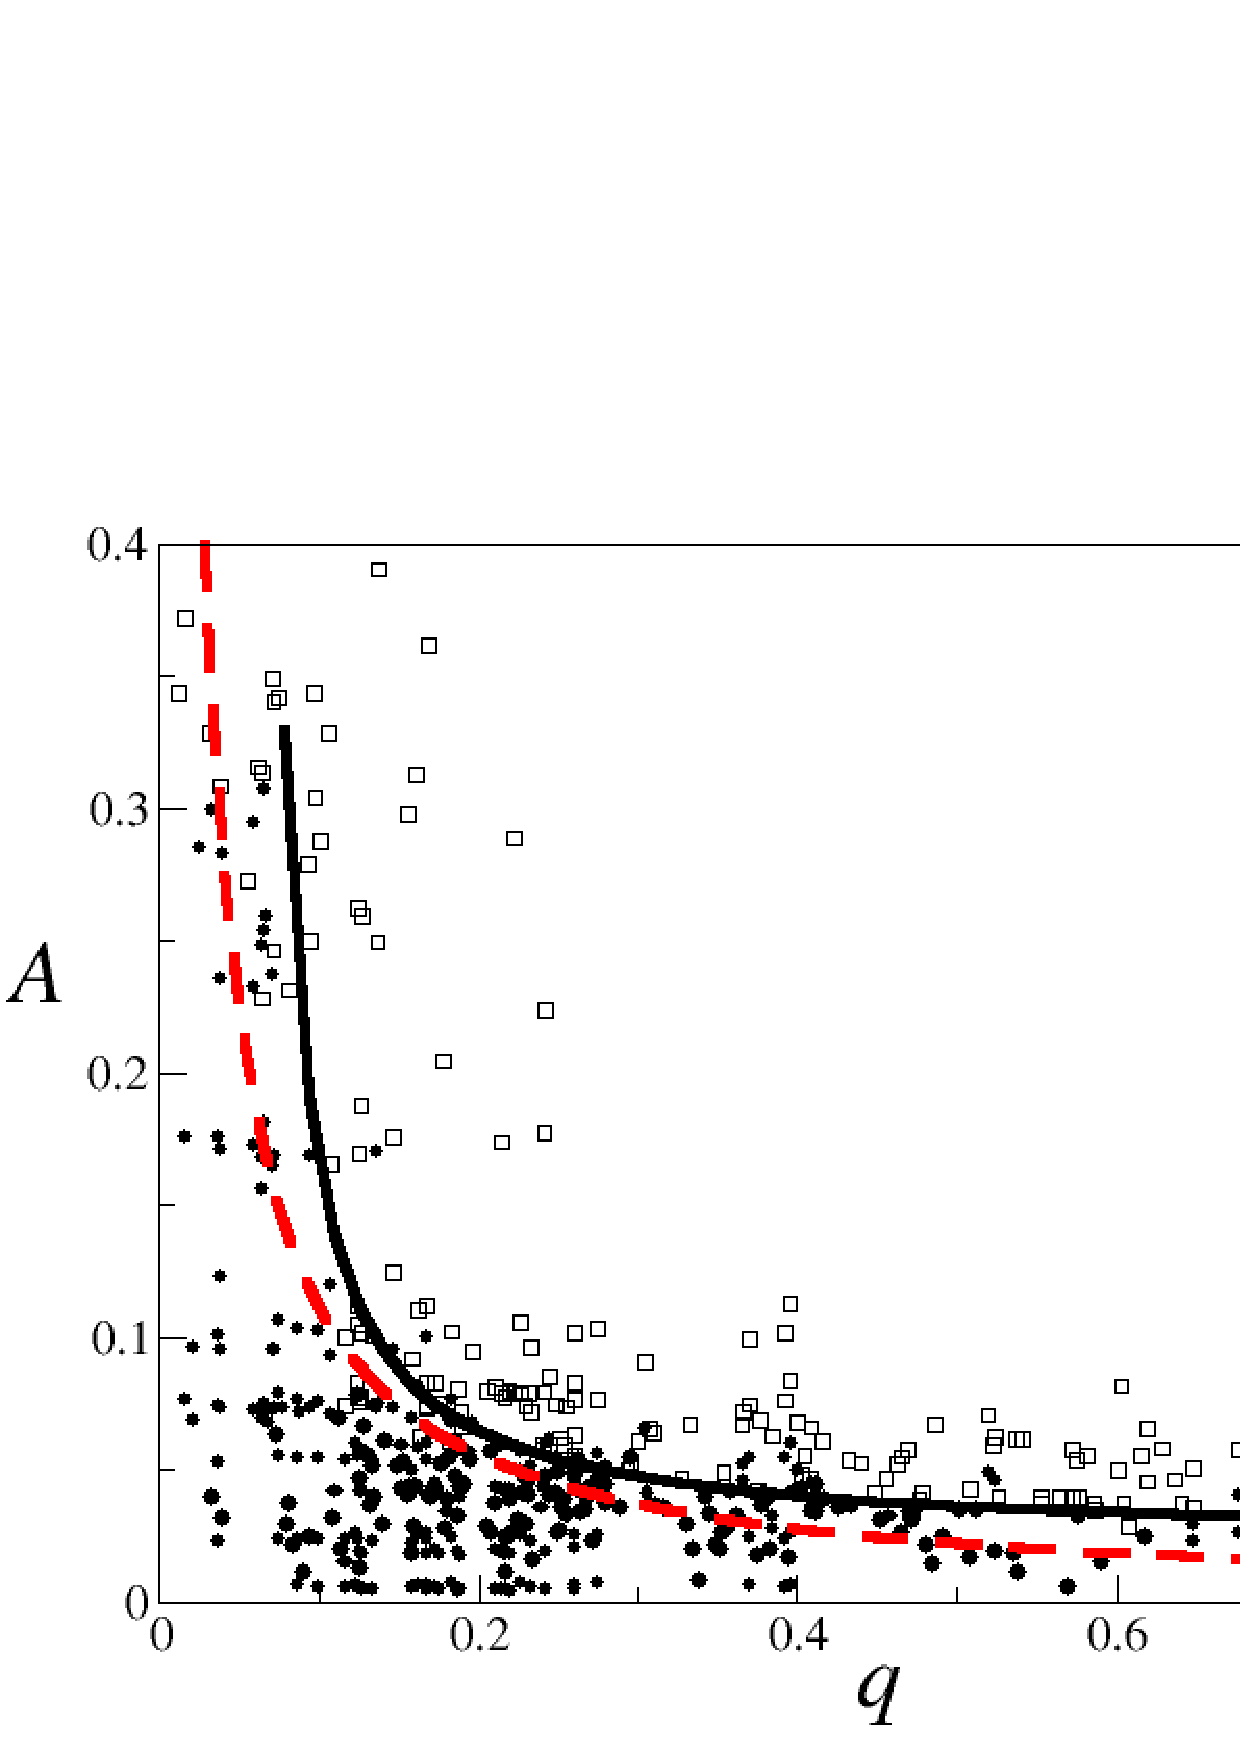
\includegraphics[width=0.8\textwidth]{polydisperse/mono1.png}\end{center}
	\caption[Crystallizability of monodisperse aspherical particles vs. $A$ and $q$]{Crystallizability of monodisperse aspherical particles characterized in terms of two shape parameters $A$ and $q$. Filled circles indicate particles that easily crystallized, while open squares indicate particles that did not.  The solid line is a guide to the eye constructed between the two distinct regions in which particles crystallize or not.  The dashed line represents a prediction of the crystallizability limit from above, $Aq = \simeq 0.011$.}\label{mono1}
\end{figure}
It is obtained by collecting 
the crystallizability of the 487 systems built out of the 487
different particle geometries we have generated across the $A$, $q$ spectrum. 
Each point in the $A$ vs $q$ diagram represents the result of a set of simulations at different pressures.
As would be expected, crystallization is favored when both $A$ and $q$ are small -- that is, 
when the particles are nearly spherical by both measures.  
A roughly inverse relationship is clearly evident; particles with large $A$ must have very small $q$ in order to have
a hope of crystallization, and vice-versa.
But more importantly, we find the existence of a clear boundary delineating the crystallizability limit 
for every possible shape generated with our model (small deviations at the interface are
likely due to finite size effects and/or the limited length of our simulations).

This is quite remarkable because it provides a very useful way of predicting whether a particular particle shape can pack into a
crystalline structure by simply measuring the experimentally accessible $A$ and $q$. 

Notice that for smaller values of $q$ our data seem to 
indicate a sharp end of the crystal boundary. We believe this to be an artifact of our particle model.
In fact, that region is where the value of $\sigma_0$ becomes sufficiently  large ($\sigma_0>0.5\sigma$)
to break the compactness of the particles generated with our method, especially those with smaller values of $N_b$. 
Furthermore, as small values of $q$ indicate a large orientational symmetry, we expect this
region to be heavily populated by specific  geometric arrangements (as discussed below), whose packing properties, at large values of $A$,
will be extremely sensitive of the particular value of $N_b$. 

As our model is intended to describe randomly shaped particles, 
our diagram does not include the results for particles designed with very specific shapes such as rods,
plates or regular polyhedral geometries that are known to crystallize. 
These particular cases would generate sharp peaks around specific values of $q$. 
Furthermore, is not clear that our two order parameters, which have after all been selected to describe asphericity, 
would be the most appropriate to study deviations from an arbitrary nonspherical designed shape. 
We therefore limited our study to $N_b >3$, to explicitly avoid trivial cases such as rod-like ($N_b=2$) and plate-like particles ($N_b=3$).

The dashed line in Figure~\ref{mono1} is the limit $Aq \lesssim 0.011$ attained in Section~\ref{sec:polydisperse}.
Although it is not a perfect division, likely due to many factors (including finite-size effects), this simple prediction provides a reasonable dividing line which would predict the crystallization or non-crystallization of 387 of the 487 systems tested, or almost 80\%.
Given the uncertainties discussed above associated with the data points,  we believe this is a remarkably good rate of success.

\section{The character of crystals of aspherical particles}

Two obvious questions present themselves in the face of these data.
The first is: what is the nature of the crystals formed when particles do crystallize; 
does the system present translational but not orientational order, as expected for $A\simeq 0$, or
does the rotational motion of the particles become restricted for large values of $A$?
The second is: what sets the boundary between the two phases;
do the particles that fail to crystallize do so because they become kinetically trapped or because of the 
lack of a stable crystal phase?
\begin{figure}
	\begin{center}\subfloat[]{
		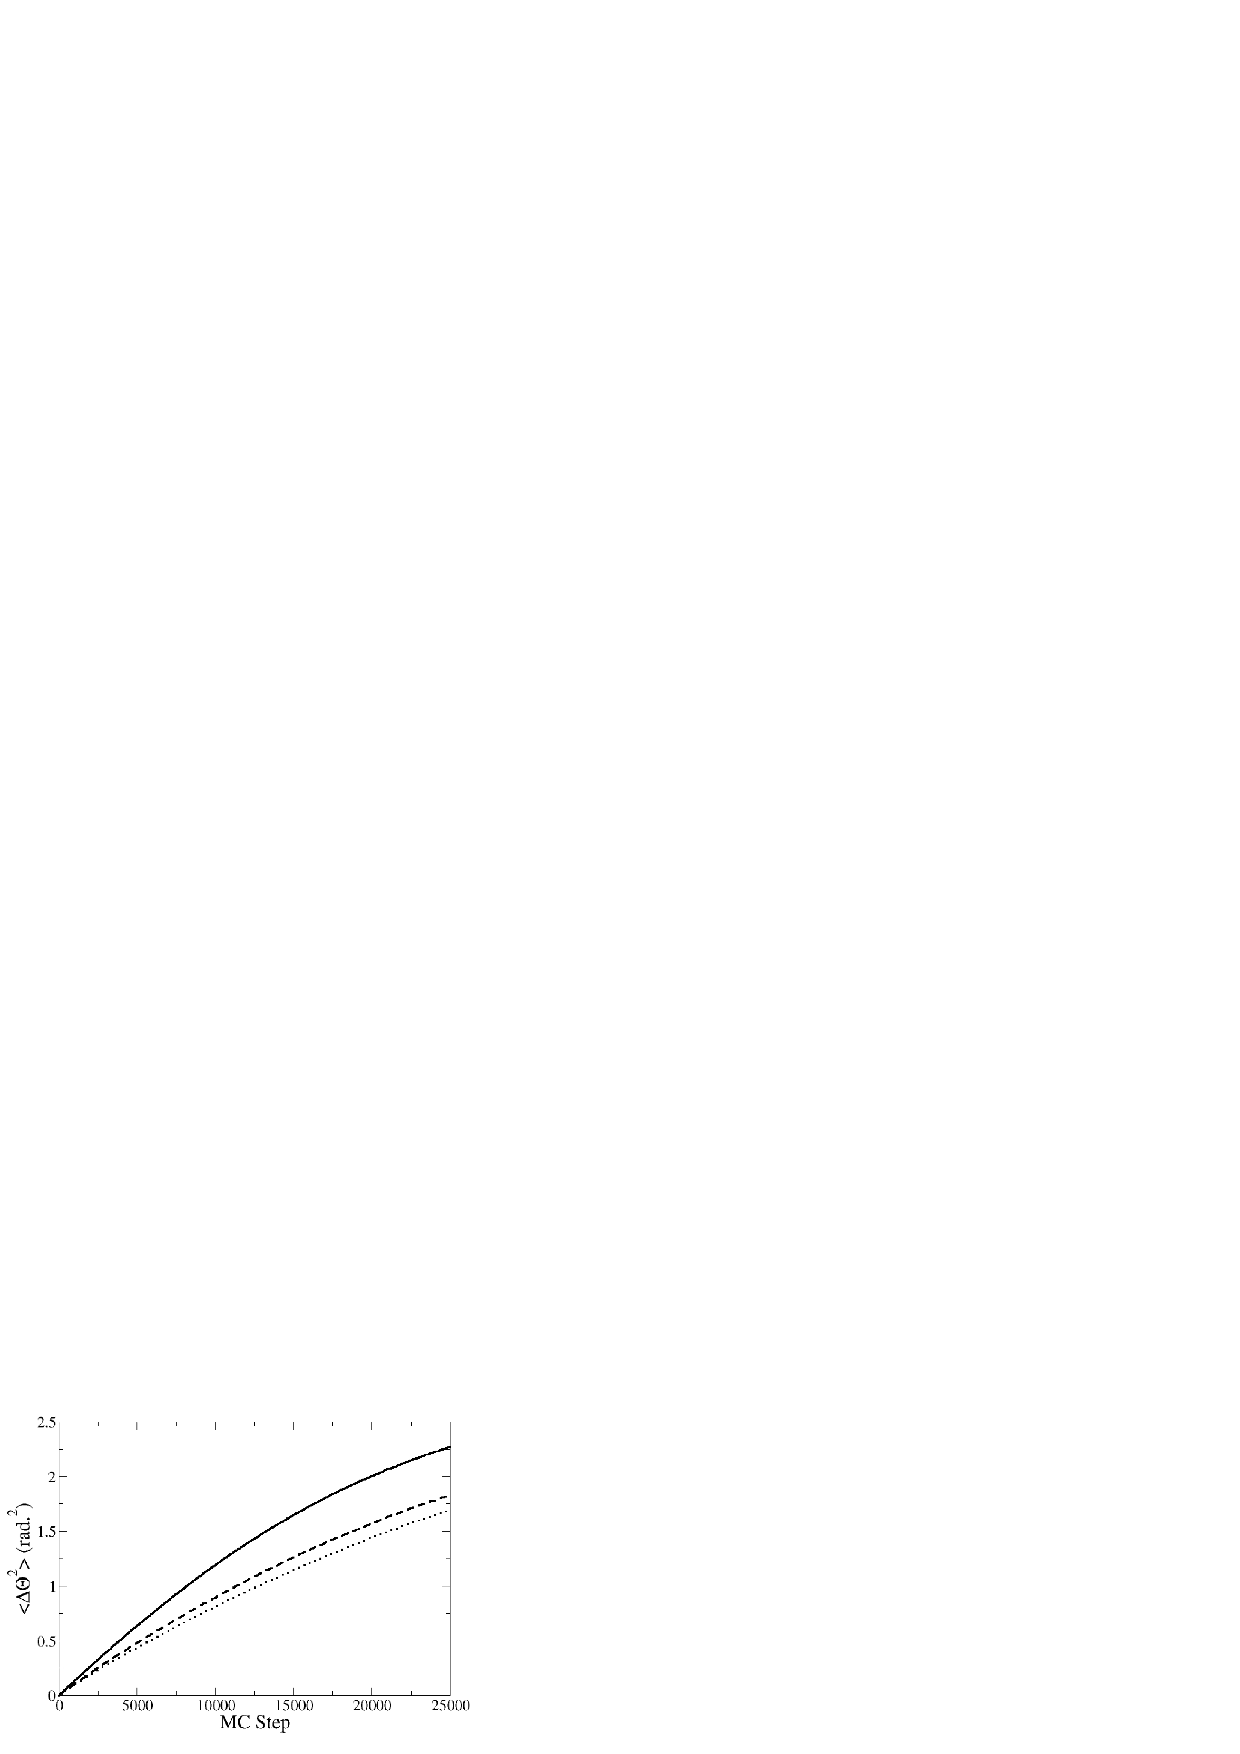
\includegraphics[width=0.6\textwidth]{disorder/rot.pdf}
		\label{rot}
	}

	\subfloat[]{
		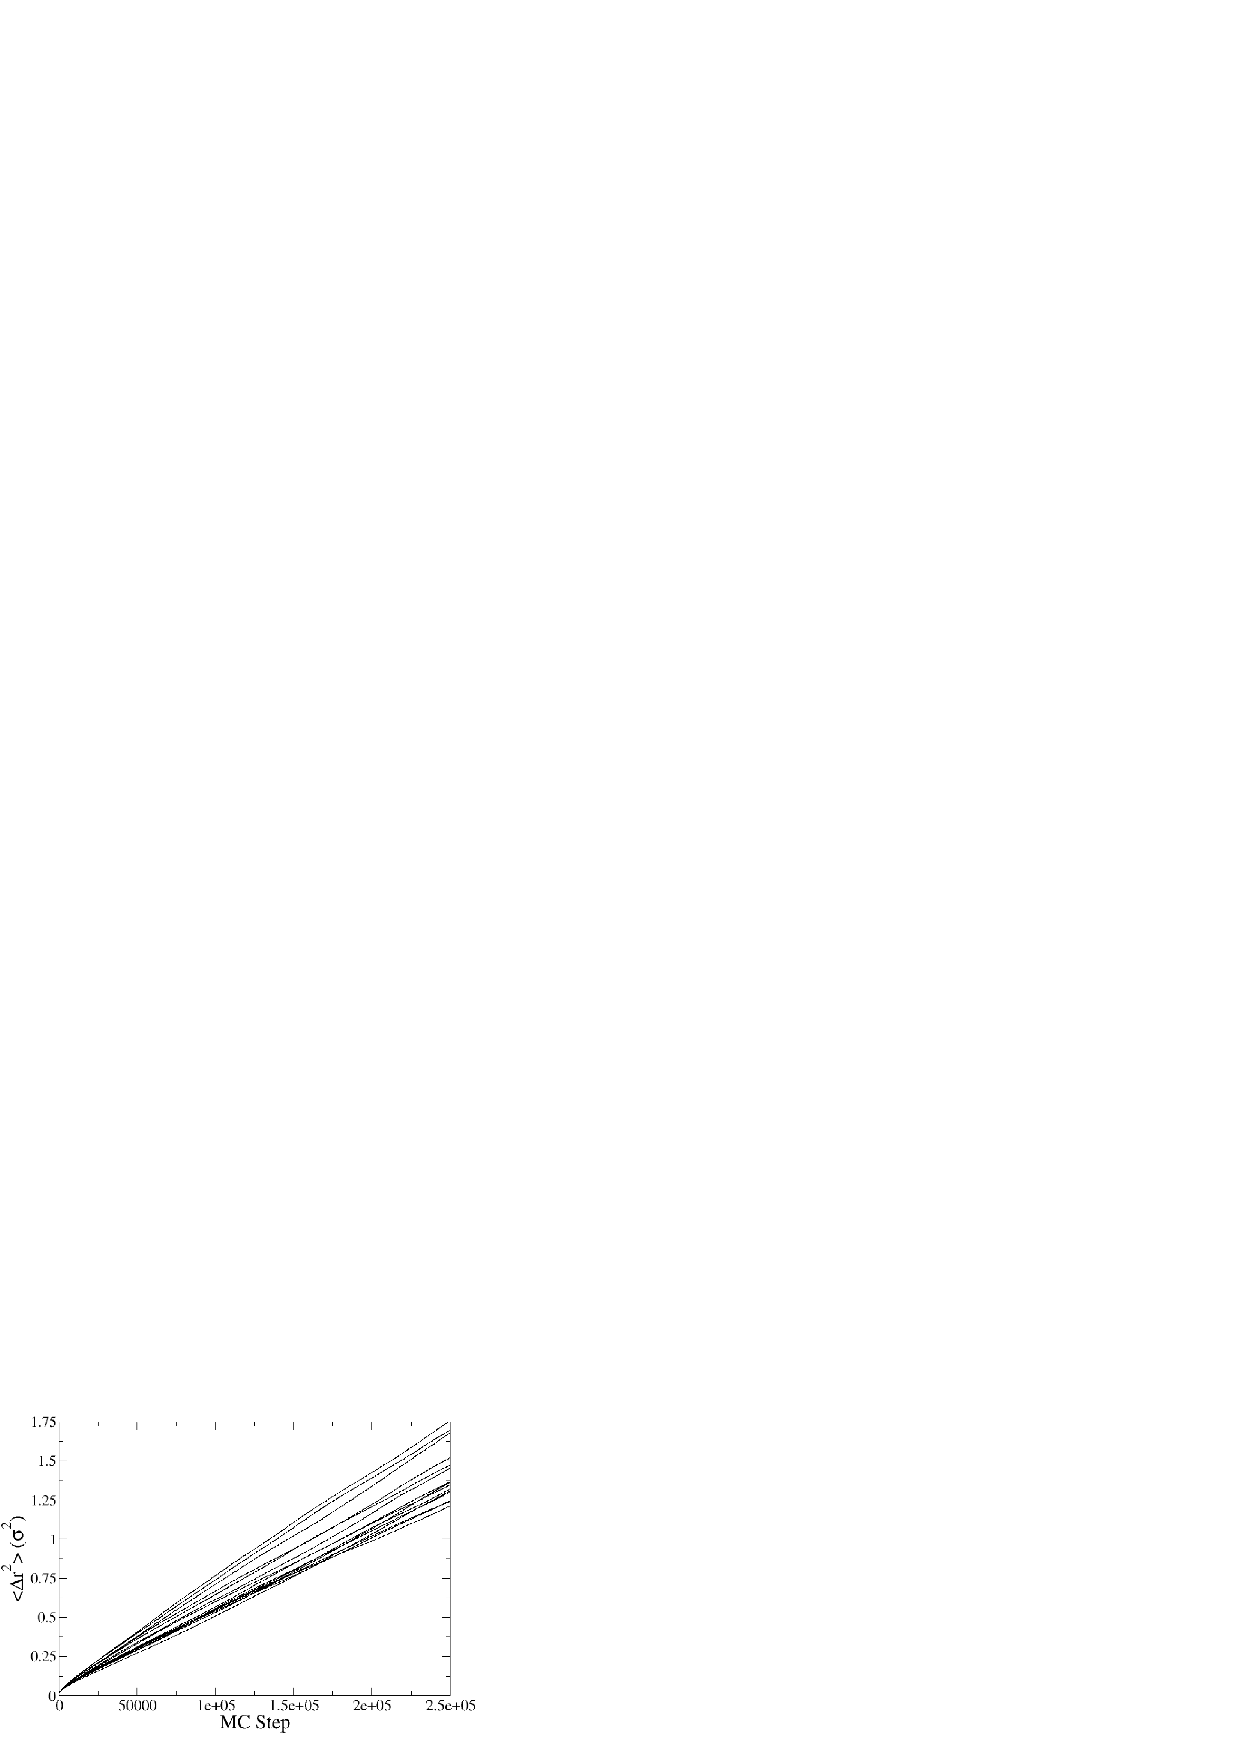
\includegraphics[width=0.6\textwidth]{disorder/trans.pdf}
		\label{trans}
	}\end{center}
	\caption[Rotational and translational diffusion for aspherical particles]{\subref{rot} Rotational mean square displacement for a subset of the particles considered. The solid line is a 
	reference for nearly spherical particles. The dashed line is the result for  those particles that  
	 crystallized and the dotted line shows $\left<\Delta\theta^2\right>$ for those that did not.
  The data were averaged over 20 realizations in each region under the same pressure $P^*=20$.
\subref{trans} Translational mean square displacement for  20 different particle shapes that failed to crystallize.}\label{diff}
\end{figure}

To address the first question, we measured the rotational diffusion, $\left<\Delta\theta^2\right>$, for 20 systems 
that crystallize, all at a reduced pressure $P^* = 20$ and near the phase boundary.  As a reference 
we also plotted  $\left<\Delta\theta^2\right>$ for nearly spherical particles, obtained by setting $\sigma_0 = 10^{-4}\sigma$, 
where we know particles are free to rotate at their lattice sites.

As can be seen in Figure~\ref{rot}, we find no evidence that particles in the crystalline phase become 
orientationally arrested or manifest an orientationally anomalous behavior. The only effect is that of decreasing their diffusion constant, 
but this is expected from simple geometrical considerations. It is obvious that at very large densities, 
regardless of the specific phase a system selects, particles' orientations will manifest a glassy behavior or eventually freeze.~\cite{schweitzer} 

It is therefore of interest to also look at the dynamical
properties of those particles in systems which do not crystallize and are located 
just across the phase boundary from the ones that do crystallize. 
These results, obtained at the same reduced pressure $P^*=20$, are also shown in Figure~\ref{rot}. 
We find no signature of anomalous dynamics, neither in the rotational (Figure~\ref{rot}), nor in the translational 
(Figure~\ref{trans}) degrees of freedom; that is, such systems behave as regular fluids.

This rotational plasticity in crystals of these aspherical particles provides and explanation for why the results of the polydisperse systems studied in Section~\ref{sec:polydisperse} applied to the monodisperse systems studied in Sections~\ref{sec:disorderpress} and~\ref{sec:disorderyesno}.
The practical effect of this fact is  
that any two identical neighboring particles will typically be misoriented and face each other with random regions of their respective surfaces. 
As a consequence, their mutual interaction becomes  hardly distinguishable, on average, from that of two particles with different shape, thus explaining why monodisperse and polydisperse 
systems may indeed present analogous equilibrium properties. 

Note, however, the deviations from the predicted pattern in Figure~\ref{mono2}
 at  the extreme ends of $Aq$,  corresponding to particle shapes that have values of $q$ significantly 
different from the average $q$ of the distribution. The deviation at large $q$ is expected as the analogous behavior is observed for polydisperse systems;
as particles become more anisotropic their rotational degrees of freedom are reduced until they perfectly align in the $q\rightarrow 1$ (rod) limit, making 
the averaged random-shape argument described above inappropriate.

A  bit more surprising is the deviation for very small values of $q$, for which we find that the polydisperse system with $N_b=12$ nicely follows the master curve.
To rationalize this behavior one has to realize that for small values of $N_b$, when $q\rightarrow 0$, particles tend to acquire rather symmetric and specific geometries, such as platonic solids, which 
also require orientational ordering  to tile the space as soon as $A$ becomes sufficiently large. These specific particle shapes dominate the shape space for $q\sim 0$ and small values of $N_b$,
and lead to deviations from the inverse power law behavior.  

This result is by no means conclusive, as a thorough investigation of this last point would require larger system sizes 
and an event-driven dynamics of the components.  Our results seem to suggest that what sets the location of 
the phase boundary is not a sudden slowdown of the dynamics of the system, but more likely
 an increase of the Gibbs free energy difference between the crystalline  and the fluid phase, analogous to
that found for polydisperse spherical particles~\cite{frenkel2}. 
It would be interesting to investigate the equilibrium properties and the stability of 
candidate crystalline structures for different values of $A$ and $q$ to investigate whether our boundary line 
coincides with the onset of crystal instability, but for the reasons given above, we have not attempted to do so.


\section{Conclusions}

To conclude, out data represent a first step in attempting to understand how deviations from asphericity affect the thermodynamics of crystallization of particle systems.
Our results show  that the coexistence pressure of systems of monodisperse and shape-polydisperse particles is remarkably well-described, within the limits described above,   
 by a simple first order Taylor expansion in terms of $Aq$, $\frac{p^* - p^*_{HS}}{p^*_{HS}} = \alpha Aq + ...$

Apart from the details concerning the dynamics of these systems, our results show that, for aspherical particles,
shape and crystallizability can be directly and easily correlated when particles are characterized in terms of their
asphericity via $q$ and $A$. Our data suggest precise limits for the manufacture of nanocomponents expected to crystallize, which should be experimentally testable,
and may have important implications for the problem of protein crystallization. 
The latter system is clearly far more complex  than the one explored here,
since not only shape, but also interparticle direct interactions (which are not necessarily isotropic), 
are responsible for the organization of proteins into large macroscopic crystals. Nevertheless, it would be
interesting to systematically explore to what extent  a similar correlation exists in this case.   

Finally, a further avenue of study, and one that is vital to truly understanding phenomena surrounding crystallization of these particles, has to do with the free volume available in a crystal.
As discussed in Section~\ref{sec:CNT}, the chemical potential difference between the fluid and crystalline phases, which is a vital consideration in the crystallization, is determined, in purely repulsive systems such as these, by the free volume available per particle in the crystal versus that available to the ``jammed'' fluid at the same density.

This is not a trivial quantity to compute in complicated systems such as these, and will be very sensitive to details about how, precisely, it is calculated.
For example, it might be necessary to attempt to calculate an ``accessible'' volume of each particle, in analogy to solvent-accessible volumes in proteins, which accounts for the fact that a narrow, deep cleft, for example, should have no bearing on the way in which two particles of the same size interact with each other.
However, this would be a vital step toward a complete theoretical understanding of the problem, and work in this direction is currently underway.
